\documentclass[11pt,a4paper]{article}
\usepackage[margin=2cm]{geometry}
\usepackage{amsmath,amssymb,amsfonts}
\usepackage{graphicx}
\usepackage{booktabs}
\usepackage{enumitem}
\usepackage{xcolor}
\usepackage{tikz}
\usetikzlibrary{arrows.meta,positioning,shapes.geometric,fit,calc,decorations.pathreplacing}
\usepackage{hyperref}
\usepackage{fancyhdr}
\usepackage{tcolorbox}
\tcbuselibrary{skins,breakable}
\usepackage{multicol}
\usepackage{float}

\definecolor{sslcolor}{HTML}{2196F3}
\definecolor{bfcolor}{HTML}{4CAF50}
\definecolor{enhcolor}{HTML}{FF9800}
\definecolor{asrcolor}{HTML}{9C27B0}
\definecolor{wavcolor}{HTML}{E91E63}
\definecolor{vadcolor}{HTML}{009688}
\definecolor{darkbg}{HTML}{1E1E2E}
\definecolor{lightbg}{HTML}{F5F5F5}

\newtcolorbox{modulebox}[2][]{
  colback=#2!5, colframe=#2!80!black,
  fonttitle=\bfseries, title=#1,
  boxrule=0.8pt, arc=3pt,
  breakable
}

\pagestyle{fancy}
\fancyhf{}
\fancyhead[L]{\small Edge Audio Intelligence --- Pipeline Reference}
\fancyhead[R]{\small EE678 Wavelets, IIT Bombay}
\fancyfoot[C]{\thepage}
\renewcommand{\headrulewidth}{0.4pt}

\title{\vspace{-1cm}\textbf{Edge Audio Intelligence System}\\[0.3em]
\large Pipeline Architecture \& Algorithm Reference\\[0.2em]
\normalsize EE678 --- Wavelets and Multiresolution Signal Processing}
\author{Pipeline Reference Document}
\date{March 2026}

\begin{document}
\maketitle
\thispagestyle{fancy}

%% ============================================================
\section{System Overview}
%% ============================================================

A modular, multi-resolution edge audio pipeline for real-time speech processing.
Six stages run in cascade; each stage adds keys to a shared dictionary that flows downstream.

\begin{figure}[H]
\centering
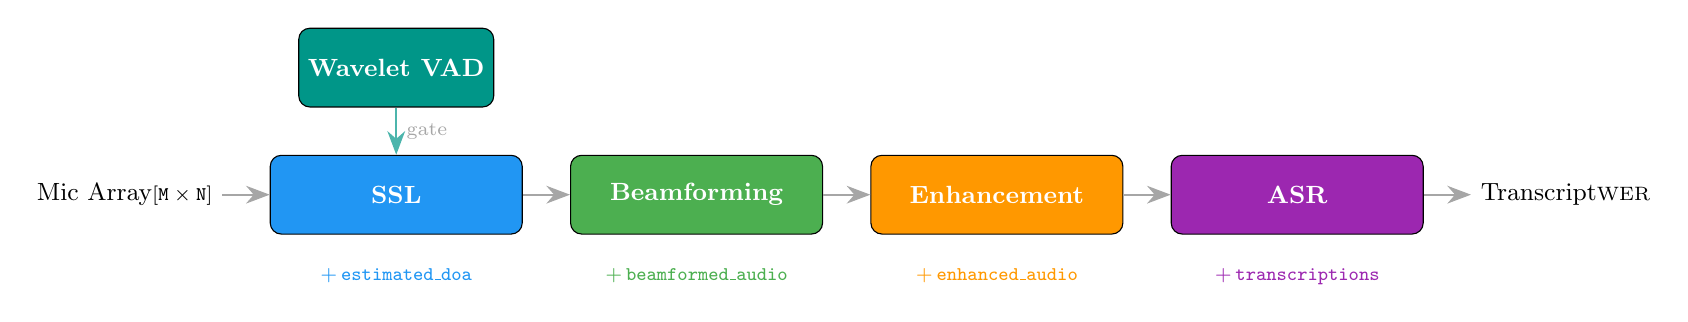
\begin{tikzpicture}[
    node distance=0.4cm and 0.6cm,
    stage/.style={draw, rounded corners=4pt, minimum width=3.2cm, minimum height=1cm,
                  font=\small\bfseries, text=white, align=center},
    arr/.style={-{Stealth[length=3mm]}, thick, gray!70},
    label/.style={font=\scriptsize, text=gray!70}
]
% Main pipeline
\node[stage, fill=sslcolor]   (ssl)  {SSL};
\node[stage, fill=bfcolor,   right=of ssl]  (bf)   {Beamforming};
\node[stage, fill=enhcolor,  right=of bf]   (enh)  {Enhancement};
\node[stage, fill=asrcolor,  right=of enh]  (asr)  {ASR};

% Arrows
\draw[arr] (ssl) -- (bf);
\draw[arr] (bf)  -- (enh);
\draw[arr] (enh) -- (asr);

% Input
\node[left=0.6cm of ssl, font=\small] (inp) {Mic Array\\[-0.1em]\scriptsize$[\texttt{M} \times \texttt{N}]$};
\draw[arr] (inp) -- (ssl);

% Output
\node[right=0.6cm of asr, font=\small] (out) {Transcript\\[-0.1em]\scriptsize WER};
\draw[arr] (asr) -- (out);

% Wavelet VAD above
\node[stage, fill=vadcolor, minimum width=2.4cm, above=0.6cm of ssl] (vad) {Wavelet VAD};
\draw[arr, vadcolor!70] (vad) -- (ssl) node[midway, right, label] {gate};

% Data keys below
\node[below=0.3cm of ssl,  font=\scriptsize, text=sslcolor]  {+\,\texttt{estimated\_doa}};
\node[below=0.3cm of bf,   font=\scriptsize, text=bfcolor]   {+\,\texttt{beamformed\_audio}};
\node[below=0.3cm of enh,  font=\scriptsize, text=enhcolor]  {+\,\texttt{enhanced\_audio}};
\node[below=0.3cm of asr,  font=\scriptsize, text=asrcolor]  {+\,\texttt{transcriptions}};

\end{tikzpicture}
\caption{V1 Cascade Pipeline. Each module appends keys to the shared data dictionary.}
\end{figure}

\noindent\textbf{Signal Model.}\quad
The $m$-th microphone receives:
\begin{equation}
x_m(t) = \sum_{s=1}^{S} h_{ms}(t) * s_s(t) \;+\; n_m(t)
\label{eq:signal}
\end{equation}
where $h_{ms}$ is the room impulse response (RIR) from source~$s$ to mic~$m$, $s_s$ is the clean source signal, and $n_m$ is additive noise.
RIRs are generated via the \textbf{Image Source Method} (pyroomacoustics).

\medskip
\noindent\textbf{Default Setup:} 4-mic linear array, 5\,cm spacing, room $6\!\times\!5\!\times\!3$\,m, $f_s = 16$\,kHz, seed~42.

%% ============================================================
\section{Stage 1 --- Sound Source Localization (SSL)}
%% ============================================================

Estimates the direction-of-arrival (DOA) $\hat{\theta}$ of each active source from the multichannel input.

%% --- GCC-PHAT ---
\begin{modulebox}[GCC-PHAT \normalfont(default)]{sslcolor}
\textbf{Idea.} Cross-correlate a microphone pair with phase-transform weighting to find the time-delay of arrival (TDOA), then convert to DOA.

\medskip\noindent
\textbf{Algorithm.}
\begin{enumerate}[nosep]
\item Select the widest-baseline mic pair (best angular resolution).
\item Cross-power spectrum with PHAT weighting:
\begin{equation}
R_{xy}(f) = \frac{X(f)\,Y^*(f)}{|X(f)\,Y^*(f)|}
\end{equation}
\item Inverse FFT to get the generalized cross-correlation:
\begin{equation}
\text{gcc}(\tau) = \text{IFFT}\{R_{xy}(f)\}
\end{equation}
\item Sub-sample peak via 3-point parabolic interpolation $\;\Rightarrow\;\hat{\tau}$ samples.
\item Convert TDOA to DOA:
\begin{equation}
\hat{\theta} = \arccos\!\left(\frac{\hat{\tau}\,c}{d\,f_s}\right), \qquad c = 343\;\text{m/s}
\end{equation}
\end{enumerate}

\noindent\textbf{Parameters:} \texttt{n\_fft}$\,=1024$.\quad
\textbf{Complexity:} $\mathcal{O}(N\log N)$ --- three FFTs.
\end{modulebox}

%% --- SRP-PHAT ---
\begin{modulebox}[SRP-PHAT]{sslcolor}
\textbf{Idea.} Steer a spatial grid of candidate directions; sum GCC-PHAT values at the corresponding TDOA for each pair. The grid maximum is the DOA.

\begin{equation}
P_{\text{SRP}}(\theta) = \sum_{\text{pairs}}\sum_{f} \text{GCC-PHAT}\!\big(\tau_{ij}(\theta),\,f\big),
\qquad \tau_{ij}(\theta) = \frac{(\mathbf{p}_i - \mathbf{p}_j)\cdot\mathbf{u}(\theta)}{c}
\end{equation}

\noindent\textbf{Parameters:} \texttt{n\_fft}$\,=1024$, grid resolution$\,=360$ (1\textdegree).\quad
\textbf{Complexity:} $\mathcal{O}(G \cdot P \cdot F)$ where $G$=grid, $P$=pairs, $F$=freq bins.
\end{modulebox}

%% --- MUSIC ---
\begin{modulebox}[MUSIC]{sslcolor}
\textbf{Idea.} Eigendecompose the spatial covariance; scan for directions whose steering vector is orthogonal to the noise subspace.

\begin{align}
\mathbf{R}_{xx}(f) &= \frac{1}{T}\sum_t \mathbf{X}(f,t)\,\mathbf{X}^H(f,t) = \mathbf{U}_s\boldsymbol{\Lambda}_s\mathbf{U}_s^H + \mathbf{U}_n\boldsymbol{\Lambda}_n\mathbf{U}_n^H \\[4pt]
P_{\text{MUSIC}}(\theta) &= \frac{1}{\mathbf{a}^H(\theta)\,\mathbf{U}_n\mathbf{U}_n^H\,\mathbf{a}(\theta)}
\end{align}

\noindent\textbf{Parameters:} \texttt{n\_fft}$\,=1024$, \texttt{n\_sources}$\,=1$, grid$\,=360$.\quad
\textbf{Complexity:} $\mathcal{O}(M^3 F + G\,M^2 F)$.
\end{modulebox}

%% ============================================================
\section{Stage 2 --- Beamforming}
%% ============================================================

Combines multichannel signals into a single enhanced channel steered towards $\hat{\theta}$.

\begin{modulebox}[Delay-and-Sum \normalfont(default)]{bfcolor}
Per-mic steering delay from the estimated DOA:
\begin{equation}
\tau_m = \frac{(\mathbf{p}_m - \mathbf{p}_{\text{center}})\cdot\mathbf{u}(\hat\theta)}{c}
\end{equation}
Fractional delay applied in the frequency domain:
\begin{equation}
X_m'(f) = X_m(f)\,\exp\!\big(-j\,2\pi f\,\tau_m / N\big)
\end{equation}
Output is the average: $\displaystyle y(t) = \frac{1}{M}\sum_{m=1}^{M} x_m(t - \tau_m)$.

\medskip\noindent
\textbf{Array gain} in spatially white noise: $G = M$ ($= 4$ for the default array).\\
\textbf{Parameters:} \texttt{use\_fractional\_delay}$\,=$\,\texttt{True}.\quad
\textbf{Complexity:} $\mathcal{O}(M\,N\log N)$.
\end{modulebox}

\begin{modulebox}[MVDR (Minimum Variance Distortionless Response)]{bfcolor}
Minimizes output power subject to unity gain in the look direction.

\begin{align}
\mathbf{R}(f) &= \frac{1}{T}\sum_t \mathbf{X}(f,t)\,\mathbf{X}^H(f,t) + \lambda\,\frac{\text{tr}(\mathbf{R})}{M}\,\mathbf{I}
\qquad\text{(diagonal loading)} \\[4pt]
\mathbf{w}(f) &= \frac{\mathbf{R}^{-1}(f)\,\mathbf{a}(f)}{\mathbf{a}^H(f)\,\mathbf{R}^{-1}(f)\,\mathbf{a}(f)} \\[4pt]
Y(f,t) &= \mathbf{w}^H(f)\,\mathbf{X}(f,t)
\end{align}

\noindent\textbf{Parameters:} \texttt{n\_fft}$\,=512$, \texttt{hop}$\,=256$, $\lambda=0.01$.\quad
\textbf{Complexity:} $\mathcal{O}(F\,M^3)$ per frame (matrix inversion).
\end{modulebox}

%% ============================================================
\section{Stage 3 --- Speech Enhancement}
%% ============================================================

Removes residual noise from the beamformed signal.

\begin{modulebox}[Spectral Subtraction \normalfont(default)]{enhcolor}
\begin{enumerate}[nosep]
\item STFT $\;\Rightarrow\; X(f,t)$.
\item Estimate noise power from first $K$ frames: $\hat{N}(f) = \tfrac{1}{K}\sum_{t=1}^{K}|X(f,t)|^2$.
\item Subtract with oversubtraction $\alpha$ and spectral floor $\beta$:
\begin{equation}
|\hat{S}(f,t)|^2 = \max\!\Big(|X(f,t)|^2 - \alpha\,|\hat{N}(f)|^2,\;\;\beta\,|X(f,t)|^2\Big)
\end{equation}
\item Reconstruct with noisy phase: $\hat{S}(f,t) = |\hat{S}(f,t)|\,e^{j\angle X(f,t)}$.
\item ISTFT $\;\Rightarrow\; \hat{s}(t)$.
\end{enumerate}

\noindent\textbf{Parameters:} \texttt{n\_fft}$\,=512$, \texttt{hop}$\,=256$, $\alpha=2.0$, $\beta=0.01$, noise frames$\,=10$, noise update rate$\,=0.98$.
\end{modulebox}

\begin{modulebox}[\textcolor{wavcolor}{$\boldsymbol\psi$}\; Wavelet Enhancement \normalfont(wavelet integration)]{wavcolor}
\textbf{Key course contribution.} Exploits the fact that speech energy concentrates in low sub-bands while broadband noise is uniformly distributed.

\begin{enumerate}[nosep]
\item \textbf{$J$-level DWT} (CDF 5/3, \texttt{bior2.2}, $J\!=\!3$):
\[
\text{signal} \;\xrightarrow{\;\text{DWT}\;}\; [cA_3,\; cD_3,\; cD_2,\; cD_1]
\]
\item \textbf{Noise estimation} via Median Absolute Deviation on finest detail:
\begin{equation}
\hat{\sigma} = \frac{\text{median}(|cD_1|)}{0.6745}
\end{equation}
\item \textbf{Level-dependent soft thresholding:}
\begin{equation}
T_j = \hat{\sigma}\,\sqrt{2\ln N}\;\cdot\;\text{scale}_j, \qquad
\widetilde{cD}_j = \text{sign}(cD_j)\,\max\!\big(|cD_j| - T_j,\;0\big)
\end{equation}
Coarser levels get lower thresholds (more speech there).
\item \textbf{Inverse DWT:}
$\;\hat{s}(t) = \text{IDWT}\big[cA_3,\;\widetilde{cD}_3,\;\widetilde{cD}_2,\;\widetilde{cD}_1\big]$
\end{enumerate}

\noindent\textbf{Sub-band frequency ranges} ($f_s = 16$\,kHz, $J=3$):

\smallskip
\begin{center}
\begin{tabular}{lcc}
\toprule
\textbf{Coefficient} & \textbf{Freq.\ Range} & \textbf{Content}\\
\midrule
$cA_3$ & 0--1\,kHz & Speech fundamentals\\
$cD_3$ & 1--2\,kHz & Speech formants\\
$cD_2$ & 2--4\,kHz & Consonants / noise\\
$cD_1$ & 4--8\,kHz & Mostly noise\\
\bottomrule
\end{tabular}
\end{center}

\noindent\textbf{Parameters:} wavelet$=$\texttt{bior2.2}, levels$=3$, mode$=$\texttt{soft}, threshold\_scale$=1.0$.\\
\textbf{Complexity:} $\mathcal{O}(N)$ total --- linear, faster than STFT's $\mathcal{O}(N\log N)$.
\end{modulebox}

%% ============================================================
\section{Stage 4 --- Automatic Speech Recognition (ASR)}
%% ============================================================

\begin{modulebox}[Whisper Offline ASR]{asrcolor}
OpenAI Whisper encoder--decoder transformer. Processes the enhanced audio in batch mode.

\medskip
\begin{center}
\begin{tabular}{lccc}
\toprule
\textbf{Model} & \textbf{Params} & \textbf{Layers} & \textbf{Use Case}\\
\midrule
tiny & 39\,M & 4 & Quick tests\\
\textbf{base} & \textbf{74\,M} & \textbf{6} & \textbf{Default (speed/accuracy)}\\
small & 244\,M & 12 & Better accuracy\\
medium & 769\,M & 24 & High accuracy\\
large & 1.55\,B & 32 & Best accuracy\\
\bottomrule
\end{tabular}
\end{center}

\noindent\textbf{Input:} 16\,kHz mono audio $\;\Rightarrow\;$ 80-channel log-mel spectrogram.\\
\textbf{Output:} text, word-level timestamps.\\
\textbf{Parameters:} \texttt{model\_size}$=$\texttt{base}, \texttt{language}$=$\texttt{en}, \texttt{device}$=$\texttt{cpu}.
\end{modulebox}

%% ============================================================
\section{Wavelet Subsystem (Course Integration)}
%% ============================================================

Four integration points ensure substantive wavelet usage for EE678:

\begin{modulebox}[\textcolor{wavcolor}{$\boldsymbol\psi$}\; Wavelet Energy VAD]{vadcolor}
Ultra-low-power voice activity detector ($<5$\,mW target). Gates the entire pipeline.

\begin{enumerate}[nosep]
\item Per-frame DWT $\;\Rightarrow\;$ sub-band energies $E(cA_3),\,E(cD_3),\,E(cD_2),\,E(cD_1)$.
\item Energy ratio:
\begin{equation}
r = \frac{E(cA_3) + E(cD_3)}{E(cD_1) + \varepsilon}
\end{equation}
Speech $\Rightarrow$ high $r$ (energy in low bands); noise only $\Rightarrow$ low $r$.
\item $\text{VAD} = \mathbf{1}[r > T]$ with minimum-duration and hangover smoothing.
\end{enumerate}

\noindent\textbf{Parameters:} frame$=$512 (32\,ms), hop$=$256 (16\,ms), $T=3.0$, hangover$=$5 frames.\\
\textbf{Complexity:} $\sim\!4N$ per DWT level $+$ energy sums. Far cheaper than STFT-based VAD.
\end{modulebox}

\begin{modulebox}[\textcolor{wavcolor}{$\boldsymbol\psi$}\; Wavelet-Initialized CNN Kernels]{wavcolor}
For the multi-stream CNN SSL (V2 scope): initialize parallel convolution kernels with Daubechies filter coefficients.

\smallskip
\begin{center}
\begin{tabular}{ccc}
\toprule
\textbf{Kernel Size} & \textbf{Wavelet} & \textbf{Filter Taps}\\
\midrule
3 & db2 & 4\\
5 & db3 & 6\\
7 & db4 & 8\\
\bottomrule
\end{tabular}
\end{center}

Each kernel gets lowpass + highpass variants; small random perturbation breaks symmetry.
Benefit: faster convergence and better-conditioned multi-scale features.
\end{modulebox}

\begin{modulebox}[\textcolor{wavcolor}{$\boldsymbol\psi$}\; Interpretability Analysis]{wavcolor}
At each pipeline stage, compute the wavelet scalogram and sub-band energies to visualize how information flows and transforms. Demonstrates that the pipeline is not a black box --- each stage has an explainable multi-resolution structure.
\end{modulebox}

%% ============================================================
\section{Evaluation Framework}
%% ============================================================

\subsection{Metrics per Stage}

\begin{center}
\begin{tabular}{llll}
\toprule
\textbf{Stage} & \textbf{Metric} & \textbf{Formula / Range} & \textbf{Goal}\\
\midrule
SSL & Angular Error & $\min(|\Delta\theta|,\;360\!-\!|\Delta\theta|)$ & $\downarrow$\\
SSL & RMSAE & $\sqrt{\frac{1}{N}\sum_i e_i^2}$ & $\downarrow$\\[3pt]
Beamforming & SI-SDR & $10\log_{10}\!\frac{\|\mathbf{s}_{\text{target}}\|^2}{\|\mathbf{e}\|^2}$ \;(dB) & $\uparrow$\\[3pt]
Enhancement & PESQ & ITU-T P.862, range $[-0.5,\;4.5]$ & $\uparrow$\\
Enhancement & STOI & Short-Time Intelligibility, range $[0,\;1]$ & $\uparrow$\\
Enhancement & SI-SDR & (same as above) & $\uparrow$\\[3pt]
ASR & WER & $\frac{S+D+I}{N_{\text{ref}}}$ \;(Levenshtein) & $\downarrow$\\[3pt]
System & RTF & processing time / audio duration & $<\!1$\\
\bottomrule
\end{tabular}
\end{center}

\noindent\textbf{SI-SDR detail:}\quad
$\mathbf{s}_{\text{target}} = \frac{\langle\hat{s},\,s\rangle}{\|s\|^2}\,s$,\quad
$\mathbf{e} = \hat{s} - \mathbf{s}_{\text{target}}$.

\subsection{SNR $\times$ RT60 Evaluation Grid}

Every module comparison runs on this standardized grid:

\begin{center}
\begin{tabular}{lccc}
\toprule
& \textbf{SNR\,=\,30\,dB} & \textbf{SNR\,=\,15\,dB} & \textbf{SNR\,=\,5\,dB}\\
\midrule
RT60\,=\,0.0\,s & LL (easy) & & HL (noisy)\\
RT60\,=\,0.3\,s & & $\bullet$ &\\
RT60\,=\,0.6\,s & & $\bullet$ &\\
RT60\,=\,0.9\,s & & $\bullet$ &\\
RT60\,=\,1.2\,s & & $\bullet$ &\\
RT60\,=\,1.5\,s & LH (reverb) & & HH (hard)\\
\bottomrule
\end{tabular}
\end{center}

\noindent Corner cases (LL, HL, LH, HH) are used for quick checks; the full $3\!\times\!6 = 18$ grid for thorough evaluation.

%% ============================================================
\section{Testbench \& Simulation}
%% ============================================================

\begin{itemize}[nosep]
\item \textbf{RIR generation:} Image Source Method via \texttt{pyroomacoustics.ShoeBox} with RT60-based absorption.
\item \textbf{Mic presets:} Linear (4 mic, 5\,cm), circular (4 mic, 4.25\,cm radius), phone (2 mic, 7\,cm), smart speaker.
\item \textbf{Noise types:} white, babble, from file. Mixed at target SNR.
\item \textbf{Sources:} speech (from LibriSpeech), sine, chirp, white noise.
\item \textbf{Reproducibility:} seeded RNG per scene; full config logged as JSON.
\end{itemize}

%% ============================================================
\section{Pipeline Orchestration}
%% ============================================================

\begin{itemize}[nosep]
\item \textbf{CascadePipeline:} Sequential module chain. Calls \texttt{module.process(data)} for each stage. Records per-module timing.
\item \textbf{ExperimentRunner:} Generates scenes $\to$ runs pipeline $\to$ evaluates metrics $\to$ saves JSON $\to$ appends to \texttt{RESEARCH\_LOG.md}.
\item \textbf{Data contract:} Every module receives and returns a \texttt{Dict[str, Any]}. Keys are standardized (Section~1 diagram). Modules only \emph{add} keys; never remove.
\end{itemize}

%% ============================================================
\section{Default Pipeline Configuration}
%% ============================================================

\begin{center}
\small
\begin{tabular}{lll}
\toprule
\textbf{Parameter} & \textbf{Value} & \textbf{Source}\\
\midrule
Sample rate & 16\,kHz & \texttt{default.yaml}\\
Room & $6\times5\times3$\,m & \texttt{default.yaml}\\
RT60 & 0.3\,s & \texttt{default.yaml}\\
SNR & 15\,dB & \texttt{default.yaml}\\
Mic array & 4-mic linear, 5\,cm & \texttt{default.yaml}\\
\midrule
SSL & GCC-PHAT, \texttt{n\_fft}$=$1024 & \texttt{default.yaml}\\
Beamformer & Delay-and-Sum, fractional delay & \texttt{default.yaml}\\
Enhancement & Spectral Subtraction, $\alpha\!=\!2$, $\beta\!=\!0.01$ & \texttt{default.yaml}\\
ASR & Whisper base, English & \texttt{default.yaml}\\
\midrule
Evaluation & Corner cases or full grid & \texttt{default.yaml}\\
Seed & 42 & \texttt{default.yaml}\\
\bottomrule
\end{tabular}
\end{center}

%% ============================================================
\section{Implementation Status}
%% ============================================================

\begin{center}
\begin{tabular}{lcc}
\toprule
\textbf{Component} & \textbf{V1 (Current)} & \textbf{V2 (Planned)}\\
\midrule
SSL: GCC-PHAT, SRP-PHAT, MUSIC & \checkmark & ---\\
SSL: Multi-stream CNN & --- & planned\\
Beamforming: DS, MVDR & \checkmark & ---\\
Enhancement: Spectral Sub., Wavelet & \checkmark & ---\\
Wavelet VAD, Init, Analysis & \checkmark & ---\\
Separation: Conv-TasNet & --- & planned\\
ASR: Whisper Offline & \checkmark & ---\\
ASR: Emformer Streaming & --- & planned\\
Diarization: pyannote & --- & planned\\
Feedback loop (Level 2) & --- & planned\\
\bottomrule
\end{tabular}
\end{center}

\end{document}
